
\section{Usando as frases musicais}
Quando dançamos realizamos movimentos concatenando eles um apos de outro 
para formar estruturas mais complexas;
porém nós não dançamos sem executar pausas ou 
variando aleatoriamente a velocidade e a expressividade de nossos movimentos; 
se não que procuramos que estes tenham sentido 
e inclusive trabalhamos para que nossos movimentos mostrem algum tipo de ordem ou tenham uma mensagem emocional ou simbólica.
Com este objetivo podemos agrupar nossos movimentos em ``frases coreográficas''.
\begin{definition}[Frase coreográfica (FC)]~
Este é um grupo de movimentos que expressem em conjunto uma ideia completa 
a qual tem algum tipo de indicador de inicio e final. 
\end{definition}

Assim, usando estas frases coreográficas, 
nós criamos estruturas maiores que guardam coerência entre si. 
Neste ponto percebemos que devemos escolher uma ideia a transmitir;
a eleição desta informação é pessoal, 
porém uma fonte de informação comumente selecionada é a música.
Aqui é usado o termo ``comumente'' porque mesmo se 
observamos a um par de dançarinos experimentados realizando uma coreografia e 
tiramos a música de sua dança, 
poderemos observar um sentido e estética no seus movimentos,
além de perceber uma introdução, frases, um \hyperref[ref:climax]{\textbf{clímax}}  e um final,
pois em alguns casos os dançarinos usam a música só como um marco emocional 
para transmitir a informação de uma historia que nasce na cabeça dos dançarinos;
mas é claro que quantos mais aspectos da música sejam interpretados na dança,
o produto final terá um aparência de maior musicalidade.

Uma boa escolha, quando buscamos uma dança com mais musicalidade, 
é procurar que nossas frases coreográficas 
encaixem nas frases musicais;
para conseguir isto nós primeiro devemos aprender a 
\hyperref[sec:perceberfrases]{\textbf{identificar as frases musicais}}\footnote{O 
tema da percepção de frases musicais foi tratado na Seção \ref{sec:perceberfrases}}.
A continuação presentamos uma serie de exercícios 
que nós ajudarão a desenvolver a capacidade de dançar seguindo as frases musicais 
até tornar esta atividade mais cotidiana.
\begin{example}[Dançando em frases de 4 compassos:]
\label{ex:usandofrases1}
(2 movimentos)
Primeiro escolheremos uma música com frases de 4 compassos como ``Piston de gafieira'' de Billy Blanco 
ou alguma das mostradas no Exemplo \ref{ex:frasesde4compassos}.
Logo procederemos a executar em cada frase musical uma frase coreográfica, de um total de duas;
de modo que a primeira frase coreográfica leva o nome ``FC 1'' e a segunda ``FC 2''.

Com a distribuição de tempos dos movimentos da Figura \ref{fig:frasecoreografica0}  
podemos escolher distintos tipos de movimentos para as frases coreográficas, 
como\footnote{Sim 
se quer agregar um pouco mais de complexidade ao exercício,
pode-se dar palmas no primeiro tempo de cada frase musical.}:
\begin{itemize}
\item \textbf{FC 1:} caminhar para adiante.
\item \textbf{FC 2:} caminhar para atrás.
\end{itemize}
Outra  escolha alternativa de movimentos pode ser:
\begin{itemize}
\item \textbf{FC 1:} realizar balanços.
\item \textbf{FC 2:} caminhar para adiante ou atrás. 
Se o exercício se realiza em pares o abraço de dança pode ser aberto, 
com uma caminha ao lado (de malandro). 
\end{itemize}
\end{example}


\begin{figure}[!h]
    \centering
    \href{https://drive.google.com/file/d/1bf1ubPovWLtBMlF4cHMeXXNAGH_C05kE/view?usp=sharing}{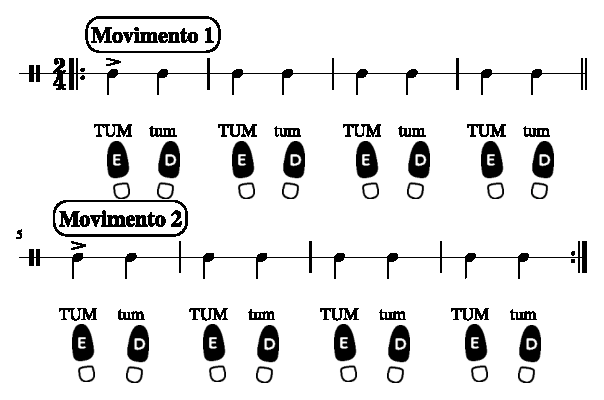
\includegraphics[width=0.9\textwidth]{chapters/cap-musicalidade/treino-fraseio0-1.eps}}
    \caption{Duas frases coreográficas de 4 compassos.}
    \label{fig:frasecoreografica0}
\end{figure}

\begin{example}[Dançando em frases de 4 compassos:](2 movimentos)
De forma similar ao Exemplo \ref{ex:usandofrases1},
usaremos uma frase coreográfica de 8 tempos com 
uma distribuição de tempos nos movimentos como mostrado na Figura \ref{fig:frasecoreografica1a}. 
Nós podemos escolher distintos tipos de movimentos para estas duas frases coreográficas, 
como\footnote{Sim 
se quer agregar um pouco mais de complexidade ao exercício,
pode-se dar palmas no primeiro tempo de cada frase musical.}:
\begin{itemize}
\item \textbf{FC 1:} realizar balanços.
\item \textbf{FC 2:} realizar cruzados.
\end{itemize}
Outra  escolha alternativa de movimentos pode ser:
\begin{itemize}
\item \textbf{FC 1:} realizar balanços.
\item \textbf{FC 2:} realizar o frente trás (básico linear).
\end{itemize}
Para ir à seguinte frase coreográfica usaremos a distribuição de tempos indicada no último compasso de cada frase 
mostrada na Figura \ref{fig:frasecoreografica1a}.
\end{example}

\begin{figure}[!h]
    \centering
    \href{https://drive.google.com/file/d/11rRCjadkiARMnrgTAQUq3A0s6xMLi5B4/view?usp=sharing}{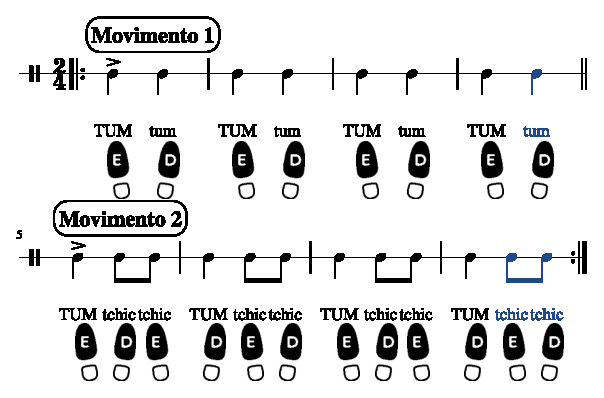
\includegraphics[width=0.9\textwidth]{chapters/cap-musicalidade/treino-fraseio1a-1.eps}}
    \caption{Duas frases coreográficas de 4 compassos.}
    \label{fig:frasecoreografica1a}
\end{figure}


\begin{example}[Dançando em frases de 4 compassos:](3 movimentos)
Primeiro escolheremos uma música com frases de 4 compassos 
como ``Disritmia'' interpretado por Martinho da Vila 
ou alguma das mostradas no Exemplo \ref{ex:frasesde4compassos}.
Logo procederemos a executar em cada frase musical uma frase coreográfica.
A primeira frase coreográfica leva o nome ``FC 1'', 
a segunda ``FC 2''  e a terceira ``FC 3''.


Com a distribuição de tempos dos movimentos da Figura \ref{fig:frasecoreografica2a}  
podemos escolher distintos tipos de movimentos para as frases coreográficas, 
assim temos\footnote{Sim 
se quer agregar um pouco mais de complexidade ao exercício,
pode-se dar palmas no primeiro tempo de cada frase musical.}:
\begin{itemize}
\item \textbf{FC 1:} realizar balanços.
\item \textbf{FC 2:} realizar cruzados.
\item \textbf{FC 3:} realizar o frente trás (básico linear).
\end{itemize}
Em ambos casos para ir à seguinte frase coreográfica usaremos a distribuição de tempos indicada no último compasso 
de cada frase mostrada na Figura \ref{fig:frasecoreografica2a}.
%\hspave{-10pt}
\end{example}

\begin{figure}[!h]
    \centering
    \href{https://drive.google.com/file/d/1fGxjpEn_EFhG5DBS7El1CiHx-oy_Ibof/view?usp=sharing}{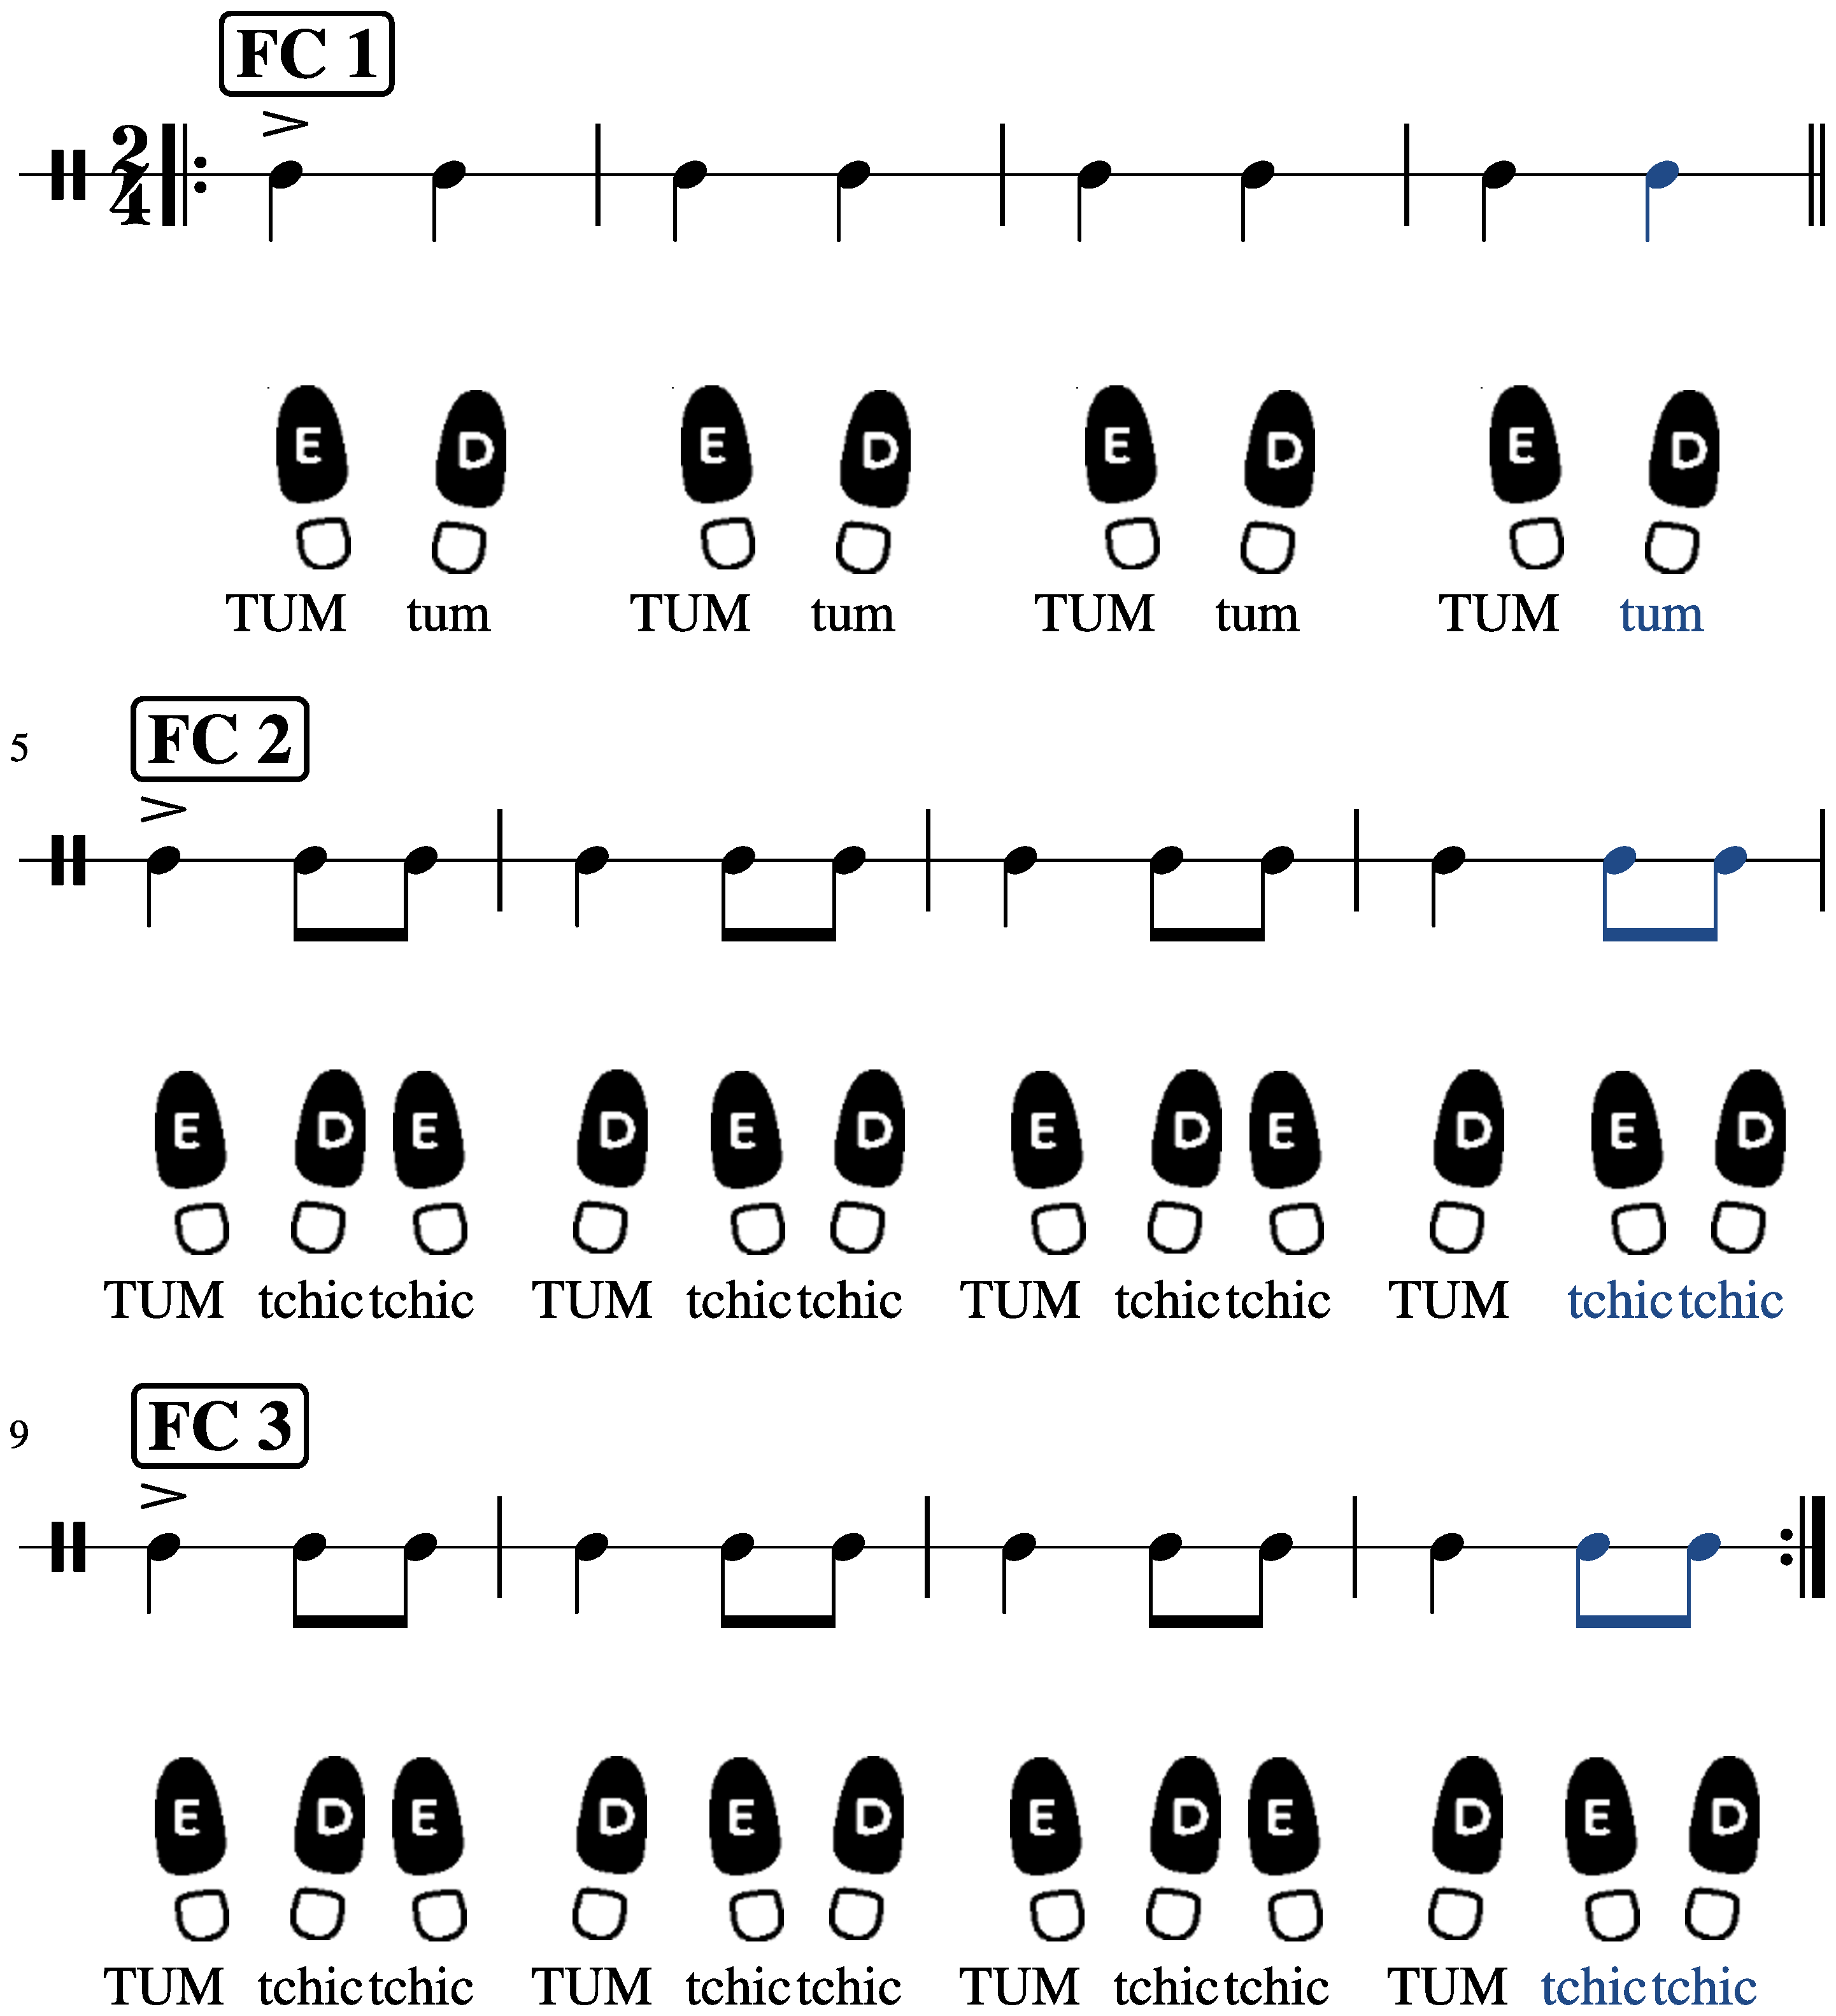
\includegraphics[width=0.9\textwidth]{chapters/cap-musicalidade/treino-fraseio2a-1.eps}}
    \caption{Duas frases coreográficas de 4 compassos.}
    \label{fig:frasecoreografica2a}
\end{figure}

\begin{comment}
\subsection{Interpretando o tipo de final da frase}
\begin{itemize}
\item Si tentamos dançar no tempo forte, conhecer a existência de ambos tipos de final de frase, 
no ajuda a ter certeza que estamos indo bem com o tempo, e que não somos nos que erramos achando o tempo forte,
e sim, que existe mais de um tipo de final de frase, e que este foi diferente, foi suspensivo.
E não nos deixaremos enganar por finais suspensivos sincopados (que parecem conclusivos),
e estaremos mais seguros de nossa dança.
\item Uma vez temos ciência da existência de ambos tipos de final, 
podemos usar suas particularidades. Por exemplo,
uma frase com final conclusivo indica o fim, literal, de uma ideia musical, 
pelo que si desejamos ter coerência com a música, 
nosso movimento e parada deve demostrar a mesma resolução,
e dar a ideia de que o relato de nossa dança acabou de expressar uma ideia completa;
para isto podemos fazer um movimento explosivo com pausa abrupta, 
ou agregar uma postura final, ou tao simples como um abraço elegante com ponto final.
Por outro lado, se o final de frase musical é suspensivo, 
a ideia transmitida tem uma sensação de pergunta,
ou de uma resposta meditativa que se apaga aos poucos e pede uma reflexão ao ouvinte,
em outras palavras um assunto não completamente  concluído.
Nesse sentido, se nosso objetivo é ter uma coerência com a música,
o relato que expressa nossa dança deve dar essa sensação de uma ideia que se apaga aos poucos,
ou de pergunta; por exemplo, isto se consegue dando um passo final em tempo forte,
seguido de movimentos corporais no lugar até a ultima nota musical.
\end{itemize}
\end{comment}

\begin{FraseOutros}{Pensamentos aleatórios}{Thomas Sowell} %RANDOM THOUGHTS
Você não pode impedir as pessoas de dizer coisas ruins sobre você. 
Tudo o que você pode fazer é torná-los mentirosos 
\cite{sowell1999barbarians}.
\end{FraseOutros}

